\section{Motion blur and deblurring}

For the synthetic experiments the clean image is the $1024\times1536$ RGB
reference from Problem 5, in $[0,1]$. I put $x$ to the right and $y$ up, and
measure the motion angle $\theta$ counter-clockwise from the $+x$ axis. In array
terms, a point $t$ along the motion sits at column $+t\cos\theta$ and row
$-t\sin\theta$ from the centre. Frequencies $f_x,f_y$ are in cycles per pixel
with the same orientation.

\subsection{Model and synthesis}

\paragraph{PSF.} During the exposure the scene moves uniformly by a total
distance $L$ along $(\cos\theta,\sin\theta)$. Each scene point is therefore
recorded with equal weight along a segment of length $L$ centred on its true
position:
\begin{equation}
h(x,y)=\frac1L\int_{-L/2}^{L/2}\delta(x-t\cos\theta,\;y-t\sin\theta)\,dt .
\end{equation}
Integrating over the plane gives $\frac1L\int_{-L/2}^{L/2}1\,dt=1$, so the blur
keeps the mean brightness. To discretise it, \code{motion\_psf} integrates $h$
over each pixel: a pixel's weight is the length of the segment inside its unit
square divided by $L$. I compute this by sampling the segment at 50 midpoints per
pixel and counting how many samples land in each pixel, then normalise the
weights to sum to exactly one. For $L=21$, $\theta=30^\circ$ the kernel is
$25\times25$ with 29 non-zero taps (\code{psf\_otf.png}). A horizontal segment
with integer $L$ becomes exactly $L$ taps of $1/L$, which the unit tests check.

\paragraph{Boundary convention.} I use circular convolution for the forward blur
and for every deconvolution: $g=\mathcal F^{-1}\{H\cdot\mathcal F\{f\}\}+n$, with
$H$ the DFT of the PSF placed with its centre at index $(0,0)$ of the image grid.
The forward model and the inverse filters are then exactly consistent, and no
pixels have to be cropped before measuring.

\paragraph{Noise.} White Gaussian noise is added to the blurred image at
\begin{equation}
\text{SNR}_\text{dB}=10\log_{10}\frac{\sum_{x,y,c}f(x,y,c)^2}{\sum_{x,y,c}n(x,y,c)^2}
\end{equation}
with $f$ the clean image, at 50, 40, 30 and 20 dB. The noise is one
standard-normal field (seed 2026) scaled to each level. The realised values are
50.000, 40.000, 30.000 and 20.000 dB (noise standard deviations 0.00159,
0.00503, 0.01589 and 0.05025), and the noisy image is not clipped.

\paragraph{OTF.} With
$\mathcal F\{h\}(f_x,f_y)=\iint h(x,y)\,e^{-j2\pi(f_xx+f_yy)}\,dx\,dy$, the delta
function collapses the double integral onto the segment. Writing
$p=f_x\cos\theta+f_y\sin\theta$,
\begin{equation}
H(f_x,f_y)=\frac1L\int_{-L/2}^{L/2}e^{-j2\pi tp}\,dt
=\frac1L\cdot\frac{e^{-j\pi Lp}-e^{j\pi Lp}}{-j2\pi p}
=\frac{\sin(\pi Lp)}{\pi Lp}=\sinc\big(L(f_x\cos\theta+f_y\sin\theta)\big).
\end{equation}
$H$ is real because the PSF is symmetric about its centre. It is zero where
$\sin(\pi Lp)=0$ with $p\ne0$, i.e.\ on the lines
\begin{equation}
f_x\cos\theta+f_y\sin\theta=\frac mL,\qquad m\in\mathbb Z\setminus\{0\}.
\end{equation}
$p$ is the component of the frequency vector $\mathbf f=(f_x,f_y)$ along the
motion direction $\mathbf u=(\cos\theta,\sin\theta)$. So neighbouring zeros are
$1/L$ apart along $\mathbf u$, and each zero set
$\{\mathbf f:\mathbf f\cdot\mathbf u=m/L\}$ is a straight line perpendicular to
$\mathbf u$: the zero lines are perpendicular to the motion direction in the
frequency plane. In words, blurring along $\mathbf u$ removes frequencies that
oscillate along $\mathbf u$, and $H$ does not change at all as you move
perpendicular to $\mathbf u$. For $L=21$ the spacing is $1/L=0.04762$
cycles/pixel.

The DFT samples $f_x=k/1536$ and $f_y=l/1024$, and the zero lines usually pass
between samples, so the sampled $|H|$ is small near them but not zero
(Table~\ref{tab:zeros}). The smallest sampled value on the grid is
$5.6\times10^{-9}$. Fig.~\ref{fig:otf} marks the sampled points closest to each
predicted line and compares $|H|$ along the motion axis with $|\sinc(Lp)|$. They
agree closely at low frequency (largest difference 0.0168 below 0.1
cycles/pixel) but differ by up to 0.51 overall. The largest difference is near a
corner of the frequency plane, at $p\approx0.5$. The PSF is sampled on the pixel
grid, so its spectrum is periodic, and $|H|$ rises again towards $p=\pm0.5$
(aliasing) while the continuous sinc keeps falling; the bumps near $p=\pm0.5$ in
the right panel of Fig.~\ref{fig:otf} show this.

\begin{table}[H]
\centering
\begin{tabular}{rrrrrr}
\toprule
$m$ & $m/L$ & samples near the line & min $|H|$ & median $|H|$ & $|\sinc|$ at $(m+\tfrac12)/L$\\
\midrule
1 & 0.04762 & 1183 & $1.33\times10^{-7}$ & $3.96\times10^{-3}$ & 0.2122\\
2 & 0.09524 & 1184 & $6.05\times10^{-6}$ & $4.54\times10^{-3}$ & 0.1273\\
3 & 0.14286 & 1182 & $5.74\times10^{-6}$ & $3.94\times10^{-3}$ & 0.0909\\
4 & 0.19048 & 1163 & $1.48\times10^{-5}$ & $1.18\times10^{-2}$ & 0.0707\\
5 & 0.23810 & 1051 & $2.64\times10^{-6}$ & $1.06\times10^{-2}$ & 0.0579\\
\bottomrule
\end{tabular}
\caption{The sampled OTF within half a frequency bin of each predicted zero line,
against the sidelobe peak between lines (\code{otf\_zeros.txt}). $m/L$ in
cycles/pixel.}
\label{tab:zeros}
\end{table}

\begin{figure}[H]
\centering
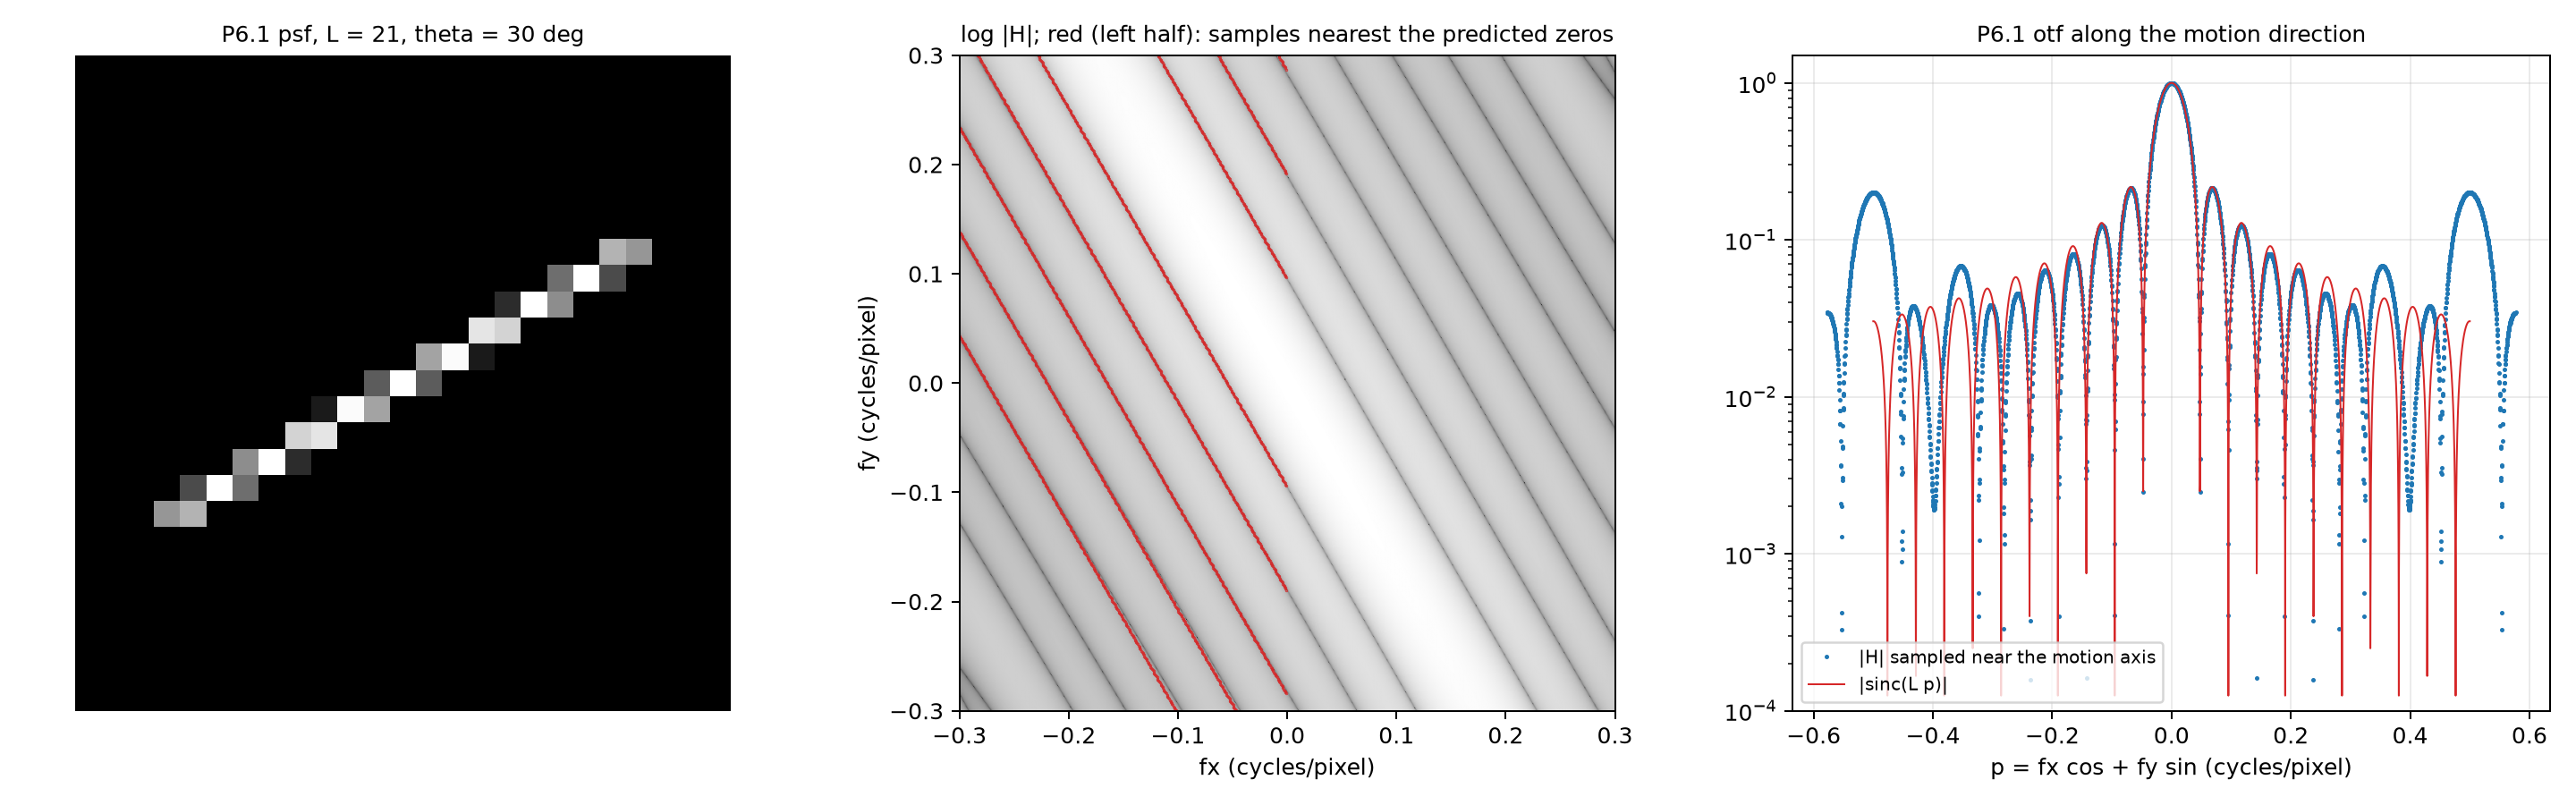
\includegraphics[width=\linewidth]{problem_6/psf_otf.png}
\caption{PSF ($L=21$, $\theta=30^\circ$); $\log|H|$ against $f_x,f_y$
(cycles/pixel) with the sampled points nearest the predicted zeros marked in the
left half; and $|H|$ along the motion direction against $|\sinc(Lp)|$.}
\label{fig:otf}
\end{figure}

\subsection{Naive inverse filtering}

I implemented $\hat F=G/H$ with a floor of $10^{-12}$ on $|H|$: values below it
are replaced by $10^{-12}$ with the phase of $H$, only to avoid dividing by an
exact zero. On this grid the floor is never reached, since the smallest $|H|$ is
$5.6\times10^{-9}$. Without noise the inverse is exact (219.25 dB, i.e.\
rounding). With noise it fails completely.

\begin{table}[H]
\centering
\begin{tabular}{rrrrrr}
\toprule
SNR (dB) & PSNR of $g$ & PSNR of $G/H$ & error near zeros & error away & ratio\\
\midrule
50 & 24.85 & 4.47 & $6.913\times10^{3}$ & $2.468\times10^{2}$ & 28.0\\
40 & 24.82 & 4.46 & $2.186\times10^{4}$ & $7.806\times10^{2}$ & 28.0\\
30 & 24.53 & 4.46 & $6.913\times10^{4}$ & $2.468\times10^{3}$ & 28.0\\
20 & 22.49 & 4.46 & $2.186\times10^{5}$ & $7.806\times10^{3}$ & 28.0\\
\bottomrule
\end{tabular}
\caption{Naive inverse filter (PSNR in dB). The error columns are the mean of
$|\hat F-F|$ (green channel) over frequencies with $|pL-m|<0.05$, $m\ne0$ (near
the zero lines) and with $|pL-m|>0.4$ (away from them)
(\code{inverse\_filter.txt}).}
\label{tab:inverse}
\end{table}

\begin{figure}[H]
\centering
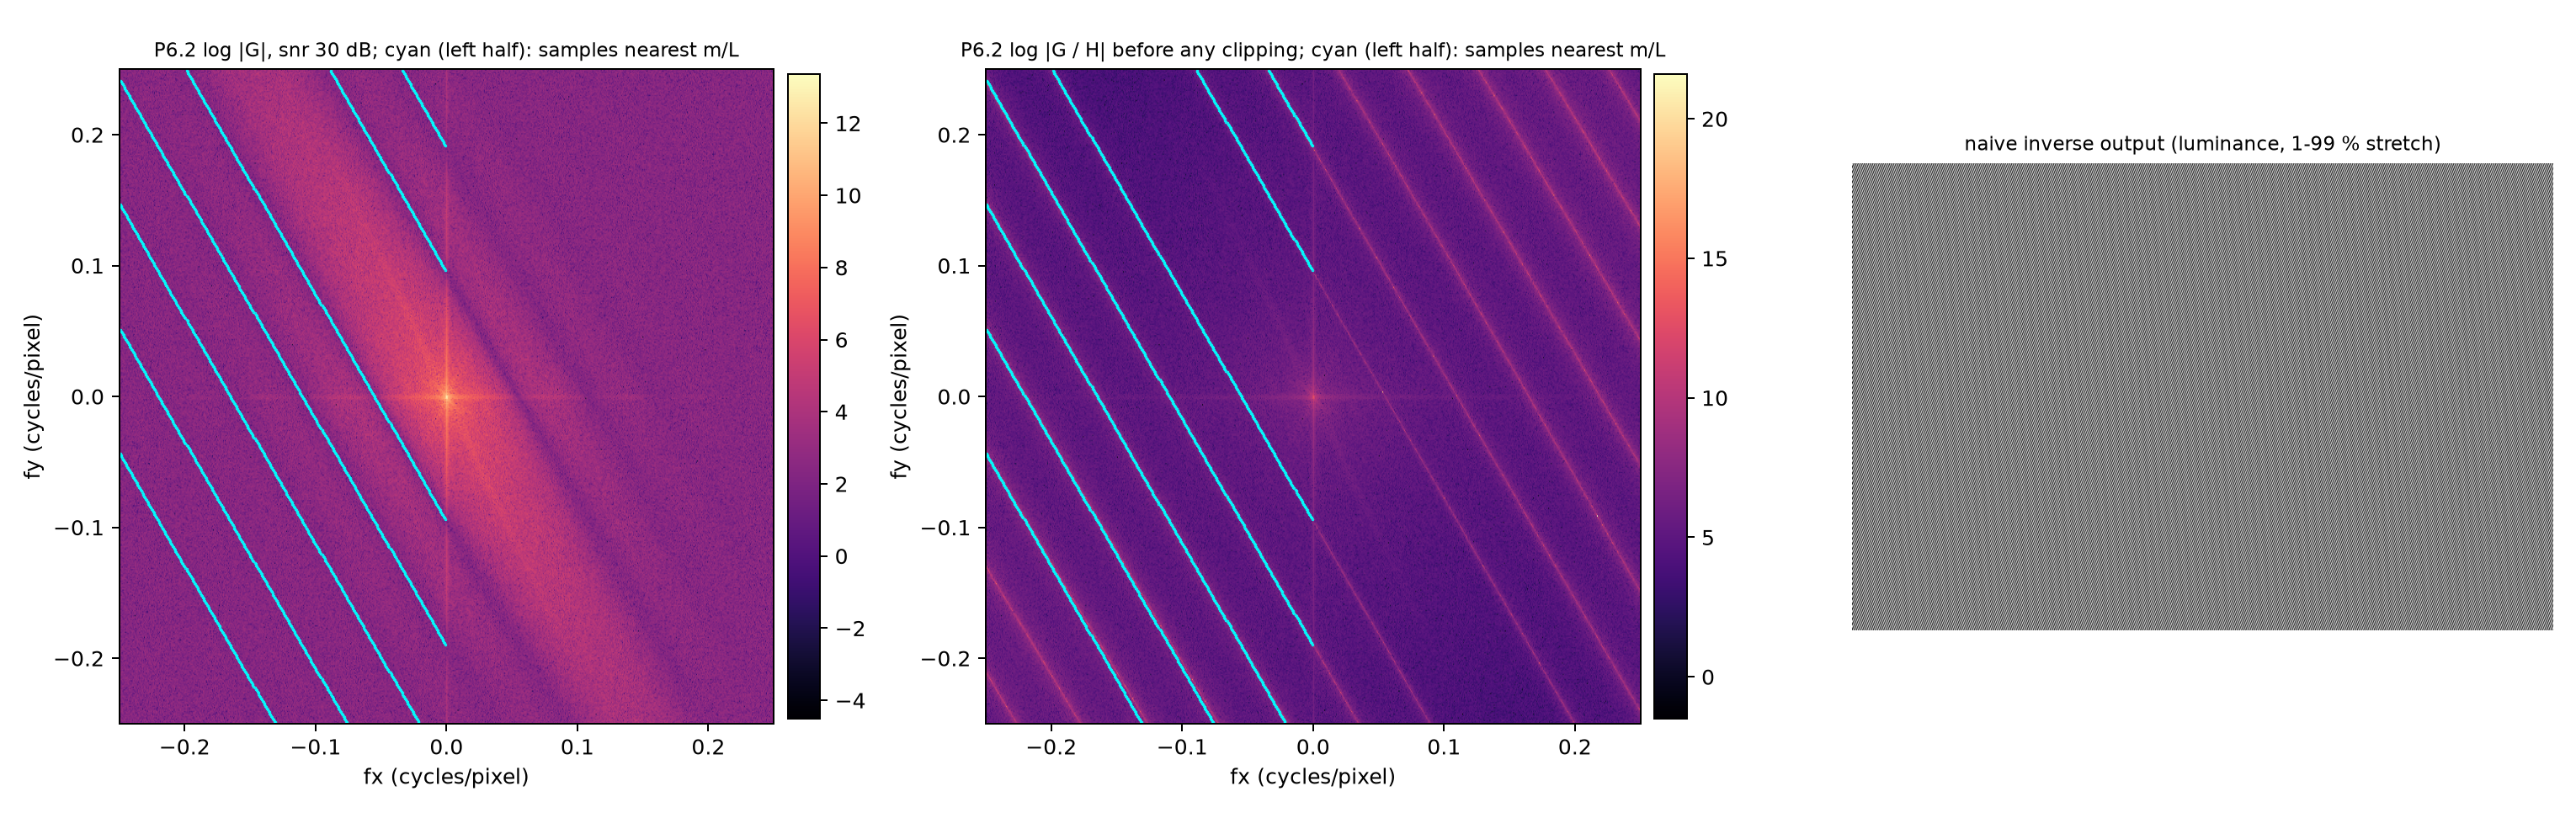
\includegraphics[width=\linewidth]{problem_6/inverse_spectrum.png}
\caption{At 30 dB: $\log|G|$, $\log|G/H|$ before any clipping, and the inverse
output, with $f_x,f_y$ in cycles/pixel. Cyan marks the sampled frequencies
nearest the predicted zeros in the left half; the right half shows the stripes
themselves.}
\label{fig:inverse}
\end{figure}

Since $G=HF+N$, the inverse gives $\hat F=F+N/H$: the image part comes back
exactly and the noise is divided by $H$. \textbf{Because $\hat F-F=N/H$, any
nonzero noise at a frequency where $|H|\to0$ is multiplied by $1/|H|\to\infty$,
so the error there can become arbitrarily large.}

In $\log|G|$ the zero lines are dark stripes perpendicular to the motion, partly
filled in by the noise floor. In $\log|G/H|$ the same lines become bright stripes
of amplified noise (Fig.~\ref{fig:inverse}). Near the zero lines the spectral
error is 28 times larger than away from them, at every SNR, because the error
$N/H$ is proportional to the noise and the ratio only depends on $|H|$. The
stripes repeat every $1/L$ along the motion direction, so the longer the blur,
the more zero lines cross the frequency plane and the more of the spectrum is
ruined. Even at 50 dB the output is pure amplified noise (4.47 dB, worse than
the blurred input).

\subsection{Wiener deconvolution}

\paragraph{Derivation.} Now $G=HF+N$ with $f$ and $n$ uncorrelated. The same
argument as in 5.1 with $\operatorname{E}[F\overline G]=\overline H S_{ff}$ and
$\operatorname{E}|G|^2=|H|^2S_{ff}+S_{nn}$ gives the linear MMSE filter
\begin{equation}
\hat F=\frac{\overline H\,S_{ff}}{|H|^2S_{ff}+S_{nn}}\,G=\frac{\overline H}{|H|^2+S_{nn}/S_{ff}}\,G
\;\approx\;\frac{\overline H(u,v)\,G(u,v)}{|H(u,v)|^2+K}.
\end{equation}
The last step replaces the frequency-dependent noise-to-signal ratio
$S_{nn}/S_{ff}$ by a single constant $K$. Images are in $[0,1]$ and the PSF sums
to one, so $H(0,0)=1$ and $K$ is a dimensionless noise-to-signal power ratio:
the DFT normalisation scales $S_{nn}$ and $S_{ff}$ by the same factor, which
cancels. Where $|H|^2\gg K$ the filter is the inverse $1/H$, and where
$|H|^2\ll K$ it tends to $\overline H/K\to0$ instead of blowing up.

\begin{table}[H]
\centering
\begin{tabular}{rrrrrrr}
\toprule
SNR (dB) & best $K$ & $10^{-\text{SNR}/10}$ & PSNR (dB) & SSIM & PSNR, $K=10^{-7}$ & PSNR, $K=1$\\
\midrule
50 & $1.58\times10^{-3}$ & $1.00\times10^{-5}$ & 31.261 & 0.8311 & 13.020 & 11.817\\
40 & $6.31\times10^{-3}$ & $1.00\times10^{-4}$ & 28.306 & 0.7003 & 7.046 & 11.817\\
30 & $2.51\times10^{-2}$ & $1.00\times10^{-3}$ & 25.825 & 0.5529 & 5.187 & 11.817\\
20 & $6.31\times10^{-2}$ & $1.00\times10^{-2}$ & 22.692 & 0.3460 & 4.679 & 11.814\\
\bottomrule
\end{tabular}
\caption{Wiener deconvolution with $K$ swept over 36 log-spaced values from
$10^{-7}$ to 1. PSNR and SSIM on outputs clipped to $[0,1]$, data range 1
(\code{k\_sweep.txt}).}
\label{tab:k}
\end{table}

\begin{figure}[H]
\centering
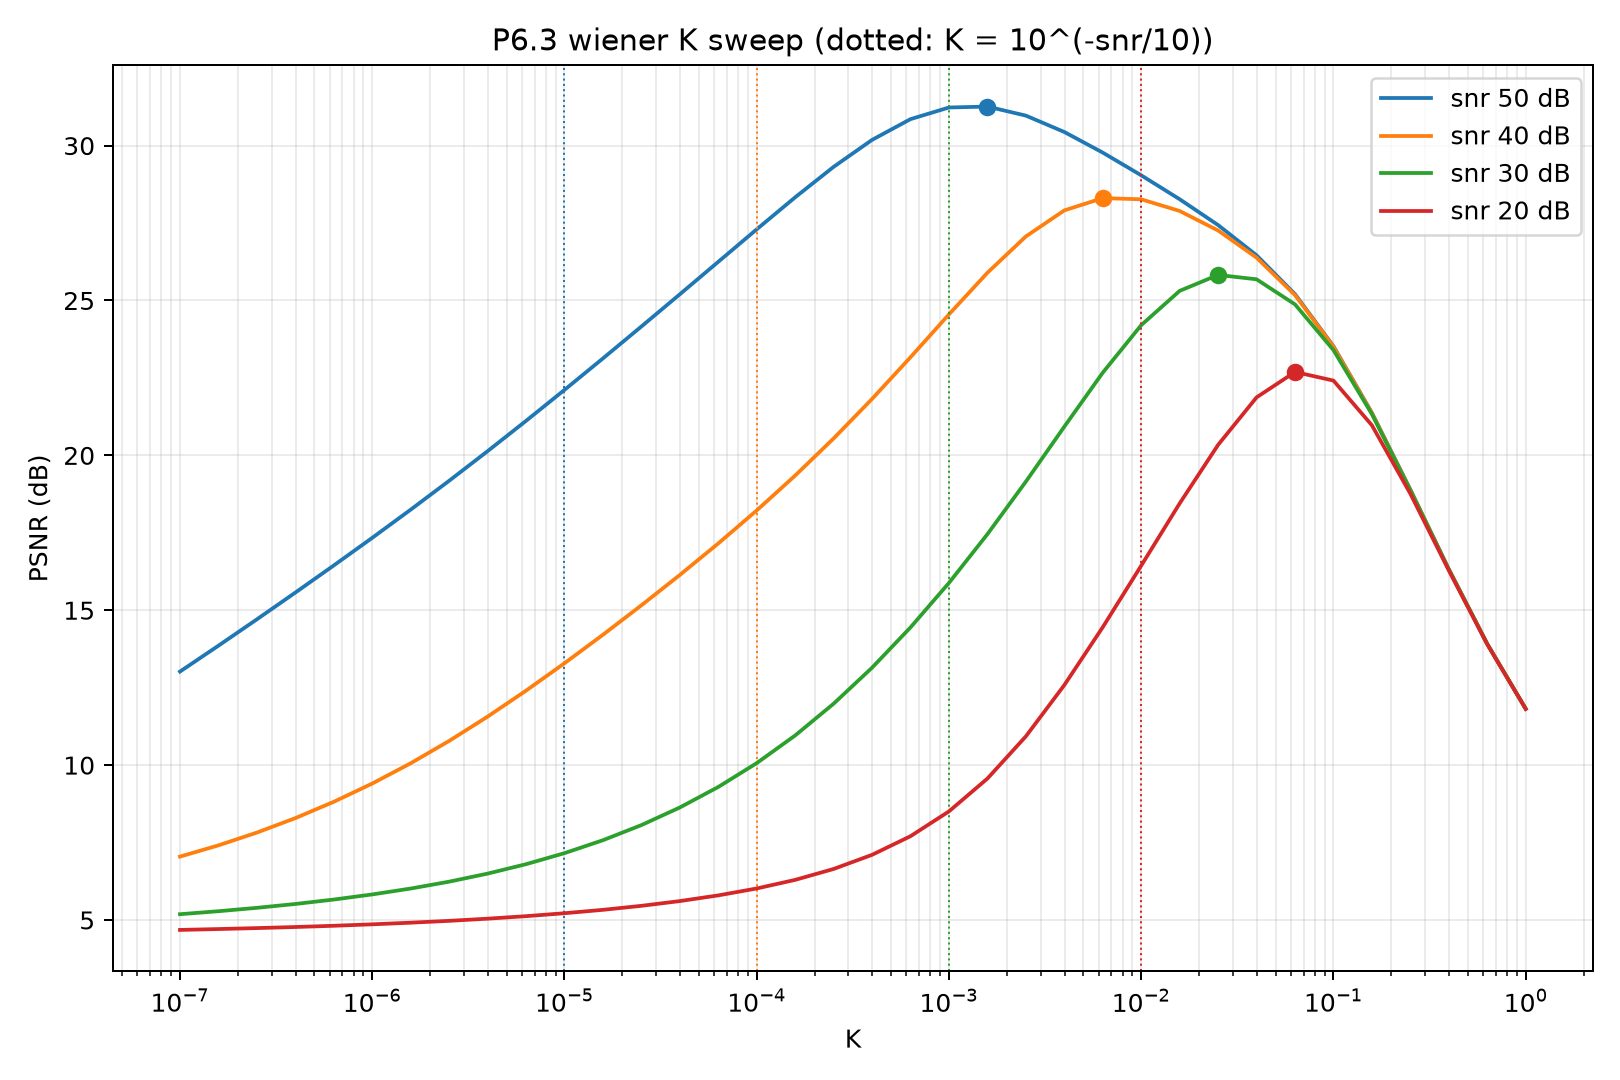
\includegraphics[width=0.68\linewidth]{problem_6/k_sweep.png}\\
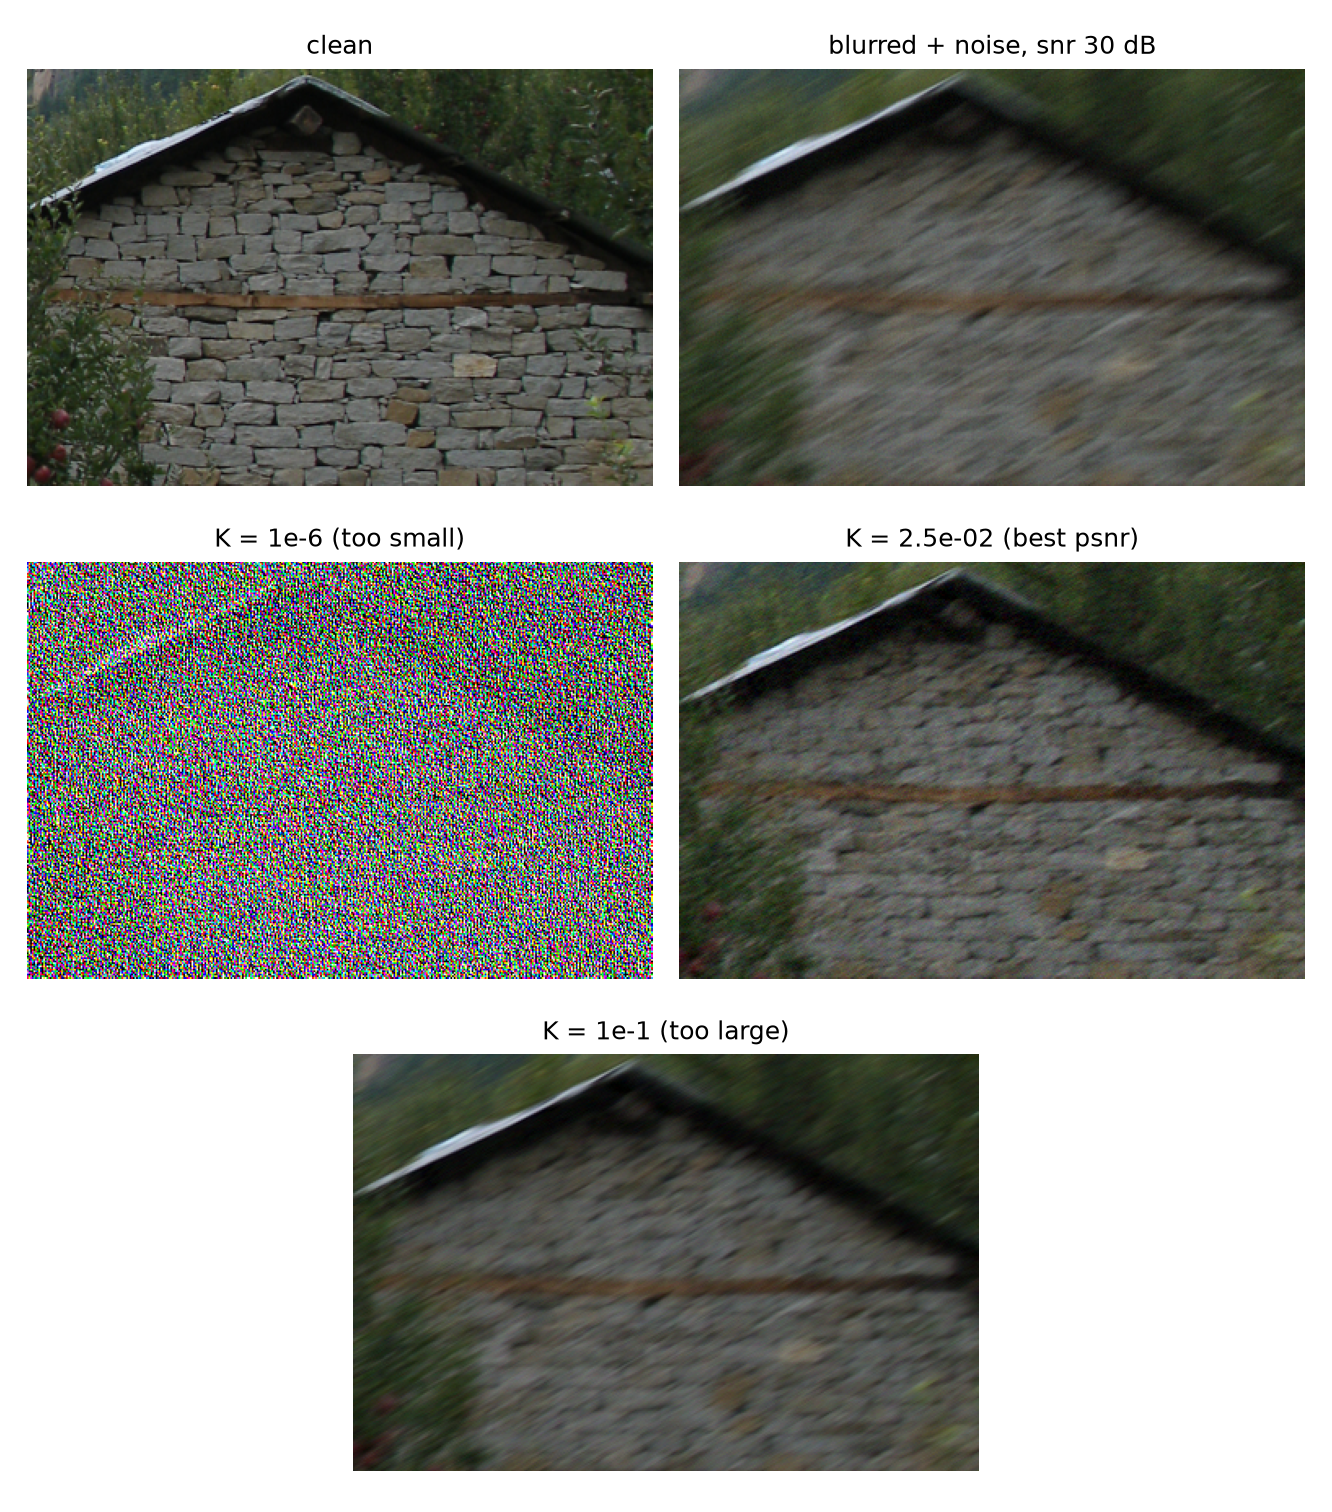
\includegraphics[width=\linewidth]{problem_6/deblurred_comparison.png}
\caption{Top: PSNR (dB) against $K$ for each SNR; dotted lines mark
$K=10^{-\text{SNR}/10}$. Bottom: roof crop at 30 dB with $K$ too small, best and
too large.}
\label{fig:k}
\end{figure}

A small $K$ brings back the inverse-filter failure: at $K=10^{-7}$ the PSNR is
4.7 to 13.0 dB and the output is dominated by amplified noise (Fig.~\ref{fig:k},
bottom). A large $K$ under-deconvolves: at $K=1$ the gain $\overline H/(|H|^2+1)$
is at most one half (exactly $1/2$ at DC), so the output is a dim, still blurred
image (11.8 dB). In between, each curve has a clear optimum, and it moves to
larger $K$ as the noise grows, from $1.6\times10^{-3}$ at 50 dB to
$6.3\times10^{-2}$ at 20 dB. The restored image gains 6.4 dB over the blurred
input at 50 dB but only 0.2 dB at 20 dB, where the noise leaves little to invert.

The best $K$ is much larger than the flat-spectrum guess $K=10^{-\text{SNR}/10}$
(the ratio of total noise power to total signal power): 158 times larger at
50 dB, falling to 6.3 times at 20 dB. $K$ stands in for $S_{nn}/S_{ff}(u,v)$ at
the frequencies where it matters, the ones where $|H|^2$ is about as large as
$K$. Those are middle and high frequencies, where a natural image has far less
power than its average (which is dominated by low frequencies), so the real
noise-to-signal ratio there is much higher than the global one. As the noise
grows, the deciding frequencies move down towards where the image power is
closer to its average, and the gap shrinks.

\subsection{Estimating and removing a real blur}

\paragraph{The photo.} I photographed the backlit keyboard of a laptop in a dim
room while moving the phone during the exposure (\code{photos/blur1.jpg},
$4032\times1816$ after the EXIF rotation). Of the four blurred shots I took, this
one has the straightest, most even streaks and the clearest blur signature. In two
of the others each key appears as several separate copies or the streaks are
kinked, and the estimator below returned a meaningless length of 4 pixels; in the
third the streaks are curved. A single straight PSF cannot describe any of those.
I also took a sharp photo of the same keyboard with the phone held still
(\code{photos/reference\_for\_blur.jpg}). It is not registered to the blurred
one, so I only use it as a control for the blur estimate, not to compute any
error. The photo is box-downsampled by 3 to $1344\times605$ so that the blur is a
few tens of pixels long and the FFTs are quick; all lengths below are at this
scale unless stated.

\paragraph{Why the stripes are perpendicular to the motion.} For a blurred photo
$|G|=|H|\,|F|$, and from 6.1 $|H|$ vanishes on the lines
$\mathbf f\cdot\mathbf u=m/L$, which are perpendicular to the motion direction
$\mathbf u$. Whatever the scene, the log spectrum therefore shows dark stripes
perpendicular to the motion, $1/L$ apart. The blur direction is the normal to the
stripes and the length is one over their spacing.

\paragraph{Estimating $\theta$ and $L$.} Taking the log of the spectrum separates
blur from scene, $\log|G|=\log|H|+\log|F|$, and $\log|H|$ repeats every $1/L$
along $\mathbf u$ (its value drops sharply at every zero line). The inverse
transform of $\log|G|$, the cepstrum, therefore has a strong negative spike at
distance $L$ from the origin in direction $\mathbf u$; this is the idea behind
Cannon's blur identification \cite{cannon}. \code{estimate\_blur} finds the most
negative cepstrum value at radius 3 to 80 in one half-plane (the cepstrum is
even) and refines its position with a three-point parabola along each axis.
Before that I multiply the image by a Hann window, so the jump at the image border
does not add a bright cross to the spectrum. On the synthetic blurred images (true
$\theta=30^\circ$, $L=21$) the estimator returns $\theta$ between $30.3^\circ$ and
$30.6^\circ$ and $L$ between 21.5 and 21.6 at all four SNRs
(\code{real\_blur.txt}). The length comes out about half a pixel long, which fits
the rasterised OTF departing from the ideal sinc at higher frequencies
(Fig.~\ref{fig:otf}).

On the photo it gives
\[
\theta=90.0^\circ,\qquad L=35.7\ \text{pixels}\ (107.2\text{ at full size}),\qquad 1/L=0.0280\ \text{cycles/pixel},
\]
with a cepstrum value of $-0.0363$ at the spike. The motion is vertical in the
frame, so the stripes should be horizontal, and they are: the red lines drawn at
$f_y=m/L$ in Fig.~\ref{fig:real-spectrum} sit on the dark bands of $\log|G|$. A
keyboard is a periodic pattern, so I checked that the spike is not caused by the
key spacing. In the sharp control photo the cepstrum at the same position is
$+0.0011$, i.e.\ there is nothing there. Its own most negative value is at a
different distance, 58.3 pixels along $90.1^\circ$, which I take to come from the
regular rows of keys.

\begin{figure}[H]
\centering
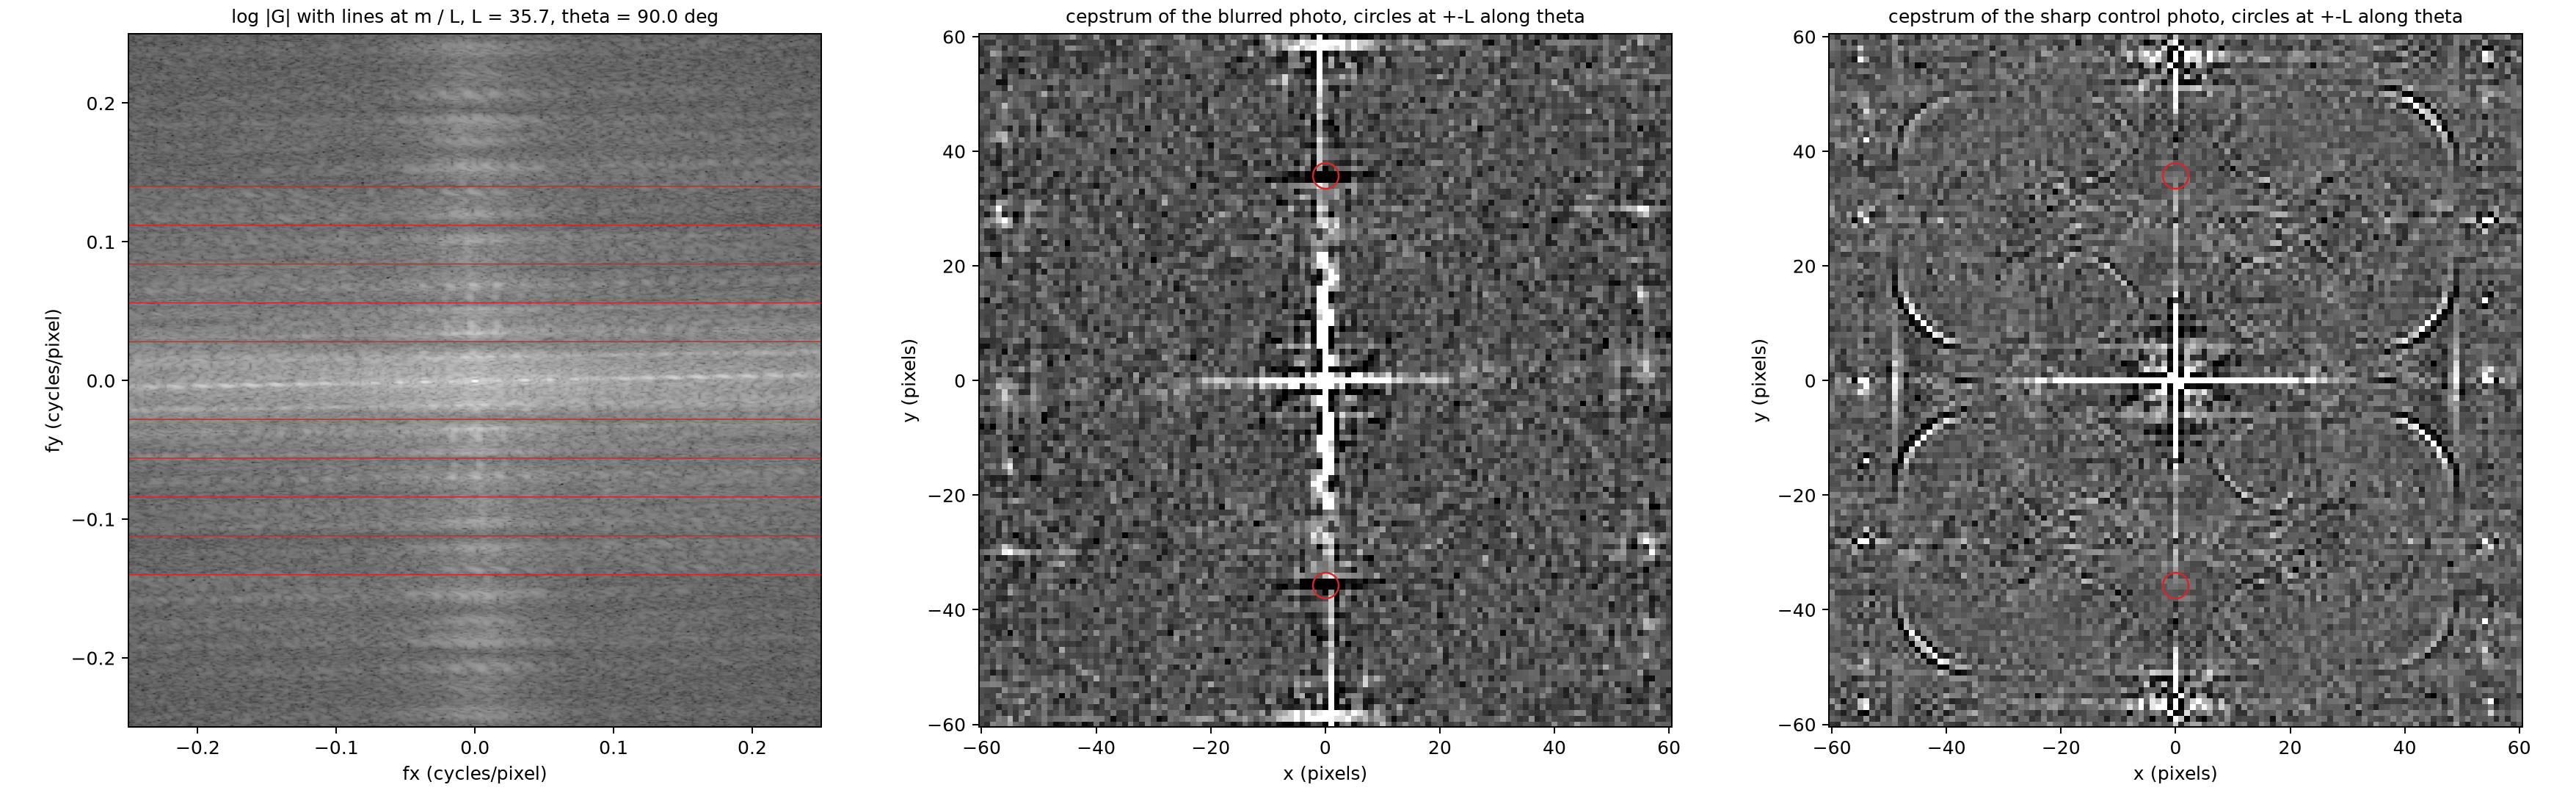
\includegraphics[width=\linewidth]{problem_6/real_blur_spectrum.png}
\caption{Left: $\log|G|$ of the Hann-windowed photo against $f_x,f_y$
(cycles/pixel), with red lines at the estimated stripe positions $f_y=\pm m/L$,
$m=1,\dots,5$. Middle: the cepstrum near the origin (pixels), with the spikes at
$\pm L$ circled. Right: the cepstrum of the sharp control photo, with nothing at
the same positions.}
\label{fig:real-spectrum}
\end{figure}

\paragraph{Deconvolution and the choice of $K$.} I built the PSF for
$\theta=90.0^\circ$, $L=35.7$ with \code{motion\_psf}, mirror-padded the photo by
$2L$ (a real blur is not circular, so circular wrap-around would add false
edges), and applied the Wiener filter for seven values of $K$. There is no clean
image to compute PSNR against, so I needed another way to pick $K$. I measured
how much the deconvolution raises the noise: the median ratio of the
plane-removed standard deviation after and before deconvolution, over the
flattest 10\,\% of the $32\times32$ tiles of the blurred photo
(Table~\ref{tab:real-k}). My rule was to take the smallest $K$ whose noise gain
is at most 2. I set this rule after a first look at a few restorations and a rough
noise check, so it states my choice precisely rather than testing it
independently. The rule gives $K=0.03$.

\begin{table}[H]
\centering
\begin{tabular}{rrrrr}
\toprule
$K$ & noise gain & outside $[0,1]$ & min & max\\
\midrule
$10^{-4}$ & 33.04 & 30.65\,\% & $-4.96$ & 10.10\\
$3\times10^{-4}$ & 20.19 & 23.23\,\% & $-4.03$ & 8.36\\
$10^{-3}$ & 11.00 & 18.10\,\% & $-2.95$ & 6.23\\
$3\times10^{-3}$ & 5.98 & 15.41\,\% & $-1.99$ & 4.45\\
$10^{-2}$ & 2.89 & 12.14\,\% & $-1.13$ & 3.05\\
$\mathbf{3\times10^{-2}}$ & \textbf{1.41} & \textbf{8.92\,\%} & $\mathbf{-0.65}$ & \textbf{2.12}\\
$10^{-1}$ & 0.62 & 5.95\,\% & $-0.29$ & 1.36\\
\bottomrule
\end{tabular}
\caption{Wiener $K$ sweep on the real photo (\code{real\_blur.txt}). Noise gain
is restored over blurred standard deviation in the flattest tiles; ``outside
$[0,1]$'' is the share of restored values below 0 or above 1. Bold: chosen.}
\label{tab:real-k}
\end{table}

\begin{figure}[H]
\centering
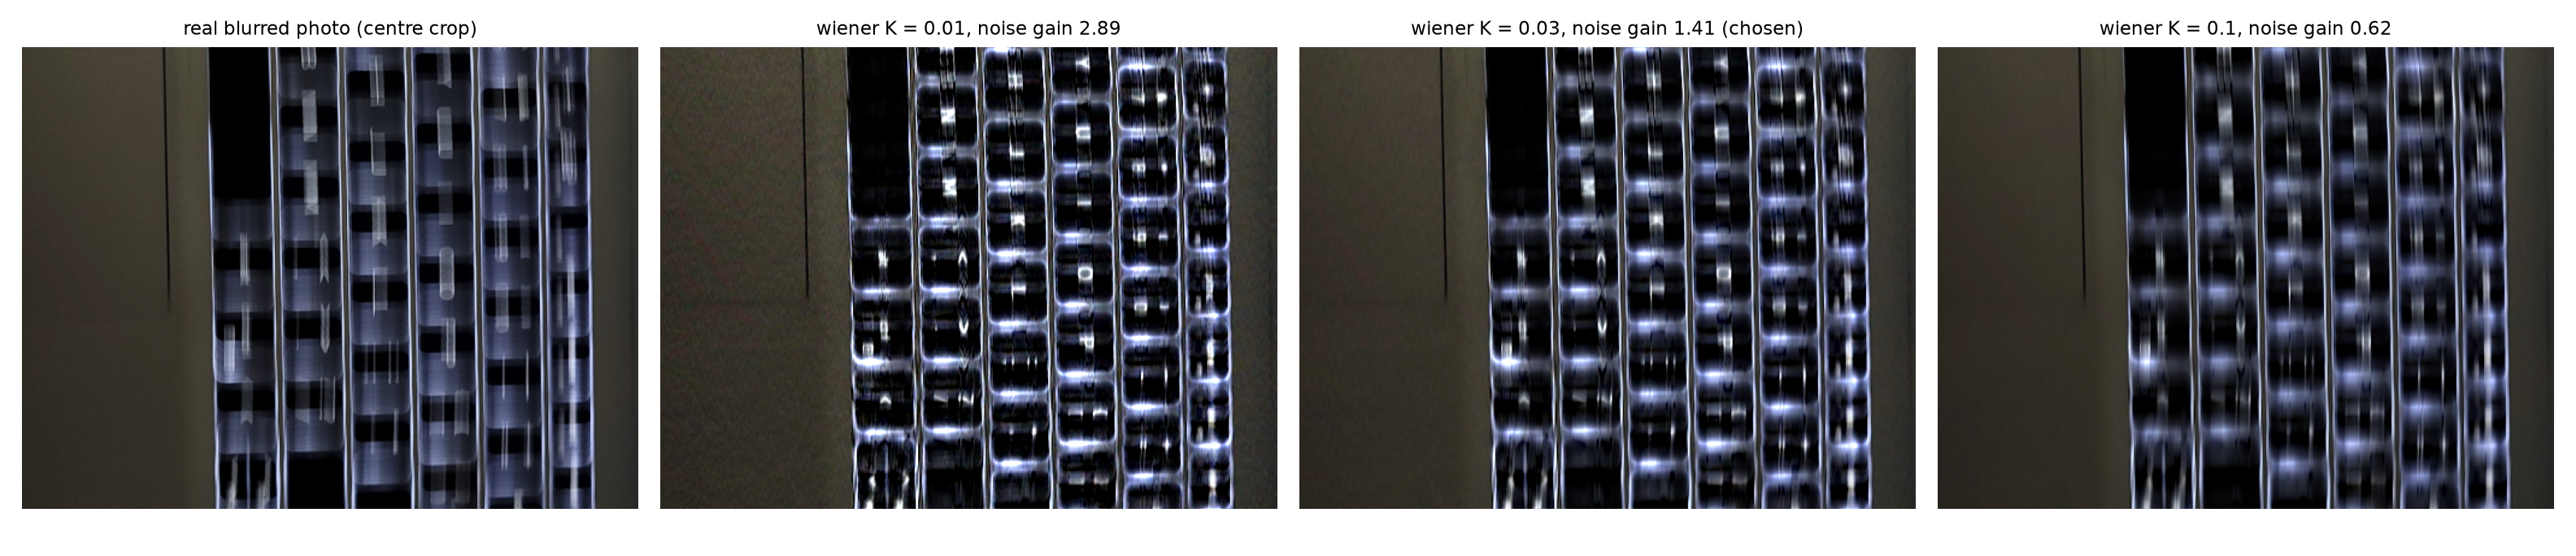
\includegraphics[width=\linewidth]{problem_6/real_blur_deblurred.png}
\caption{Centre crop of the blurred photo and the Wiener restorations with
$K=0.01$, 0.03 (chosen) and 0.1.}
\label{fig:real-deblur}
\end{figure}

In the centre of the photo the restoration works (Fig.~\ref{fig:real-deblur}).
The keys become separate rounded squares again, and several letters can be read.
$K=0.01$ recovers a little more letter detail, but its noise gain is 2.89 and
the ringing around the keys is stronger; $K=0.1$ keeps the noise below the
blurred photo's but leaves the letters smeared. The table also shows how hard the
filter pushes: even at $K=0.03$, 8.9\,\% of the restored values fall outside
$[0,1]$. Of those, 94.3\,\% are below zero, and 72.7\,\% of the negative ones
are where the blurred photo is darker than 0.1, i.e.\ ringing pushes the dark
key areas under black.

\paragraph{Artifacts and what causes them.} The restoration is not equally good
everywhere, and two things stand out: dark and bright bands below the bright
lower edge of the keyboard (Fig.~\ref{fig:real-echo}), and streaks that stay in the
top third of the frame (Fig.~\ref{fig:real-regions}). I ran two checks to find out
which of them comes from the model being wrong and which comes from the method.

\emph{The bands below the keyboard edge.} On the dark area below the brightest
edge in the photo, the restored image has a dark band 24 rows below the edge and
a bright one 40 rows below it, where the blurred photo is smooth. The pattern
repeats on a scale of about one blur length. To see whether a wrong PSF causes them, I made
a control in which the model holds exactly: my sharp photo of the same keyboard,
blurred with the estimated PSF, plus white noise at the photo's own level
($\sigma=1.21$ grey levels, measured in its flattest tiles), restored with the same
$K$. The control gets the same bands in nearly the same places (dark at 18 and
bright at 38 rows below its edge, against 24 and 40 for the photo), so they are not
a sign that the PSF is wrong. They come from inverting a blur whose transfer function
has zero lines. The model says the frequencies on the lines $f_y=m/L$ were
multiplied by zero, so the photo holds no information there, and a linear filter
can only leave those frequencies out or amplify the noise that sits there. A sharp
edge that is missing a comb of frequencies spaced $1/L$ apart comes back with
copies of itself spaced about $L$ apart. The bands are strongest at this edge
because it is the highest-contrast edge in the photo. Raising $K$ weakens them,
because the gain next to a zero line can never exceed $1/(2\sqrt K)$, but it also
sharpens less:

\begin{center}
\begin{tabular}{lrrrrr}
\toprule
& edge step & blurred & $K=0.01$ & $K=0.03$ & $K=0.1$\\
\midrule
real photo & 0.191 & 0.0057 & 0.0348 & 0.0302 & 0.0204\\
control (exact blur) & 0.038 & 0.0047 & 0.0157 & 0.0128 & 0.0094\\
\bottomrule
\end{tabular}
\end{center}

The numbers are the RMS of the row profile 14 to 94 rows below the edge (central
half of the columns, straight line removed), in luminance on $[0,1]$
(\code{real\_blur.txt}). The control's edge step is five times smaller than the
photo's, so its bands are weaker too.

\emph{The blur changes across the frame.} Running the estimator on parts of the
photo gives:

\begin{center}
\begin{tabular}{lrr}
\toprule
region & $\theta$ (deg) & $L$ (px)\\
\midrule
top third & 96.4 & 36.6\\
middle third & 90.2 & 35.6\\
bottom third & 84.9 & 36.6\\
left half & 89.2 & 35.5\\
right half & 90.4 & 36.0\\
\bottomrule
\end{tabular}
\end{center}

The length is about the same everywhere, but the direction turns by $11.5^\circ$
from the top third to the bottom third, while the left and right halves agree.
This is the real model failure in this photo: the linear, spatially invariant model
assumes one PSF for the whole image, and here the blur is different at the top and
the bottom. A small rotation of the phone about the viewing axis (a roll) during
the exposure, on top of the vertical movement, would produce exactly this pattern.
A roll by an angle $\phi$ about the frame centre moves a point at height $y$
sideways by $\phi y$, which tilts a vertical streak of length $L$ by about
$\phi y/L$. The centres of the top and bottom thirds are 448 pixels from the
middle and their streaks tilt by about $5.75^\circ$, so
$\phi\cdot448\approx35.7\tan5.75^\circ=3.6$ pixels, i.e.\ $\phi\approx0.46^\circ$.
This roll is my interpretation: it fits the measured pattern, but I did not
measure how the phone moved.

The middle third, where the local estimate agrees with the global PSF, is restored
best, while the top third keeps streaks (Fig.~\ref{fig:real-regions}, middle row).
Restoring each third with its own estimated PSF did not visibly fix the top third
(bottom row) and did not reduce the bands at the bottom edge either (0.0311 with
the bottom third's own PSF against 0.0302 with the global one). So a straight
streak at constant speed is not a good description of the local blur at the top
either. With a rolling phone the direction and speed of each point can change
during the exposure, but from this photo alone I cannot tell which of these fails.

Clipped highlights are another limit of the linear model, since a saturated pixel
no longer equals the sum of light the model assumes. Here, though, only 0.14\,\% of
the full-size pixels have a channel at 254 or 255, and only 1.8\,\% of the restored
pixels with a value outside $[0,1]$ lie within one blur length (along the motion)
of a clipped pixel, so clipping is not the main problem in this photo. Since there
is no sharp, registered original, the judgement of the restored image is visual,
and I report no PSNR or SSIM.

\begin{figure}[H]
\centering
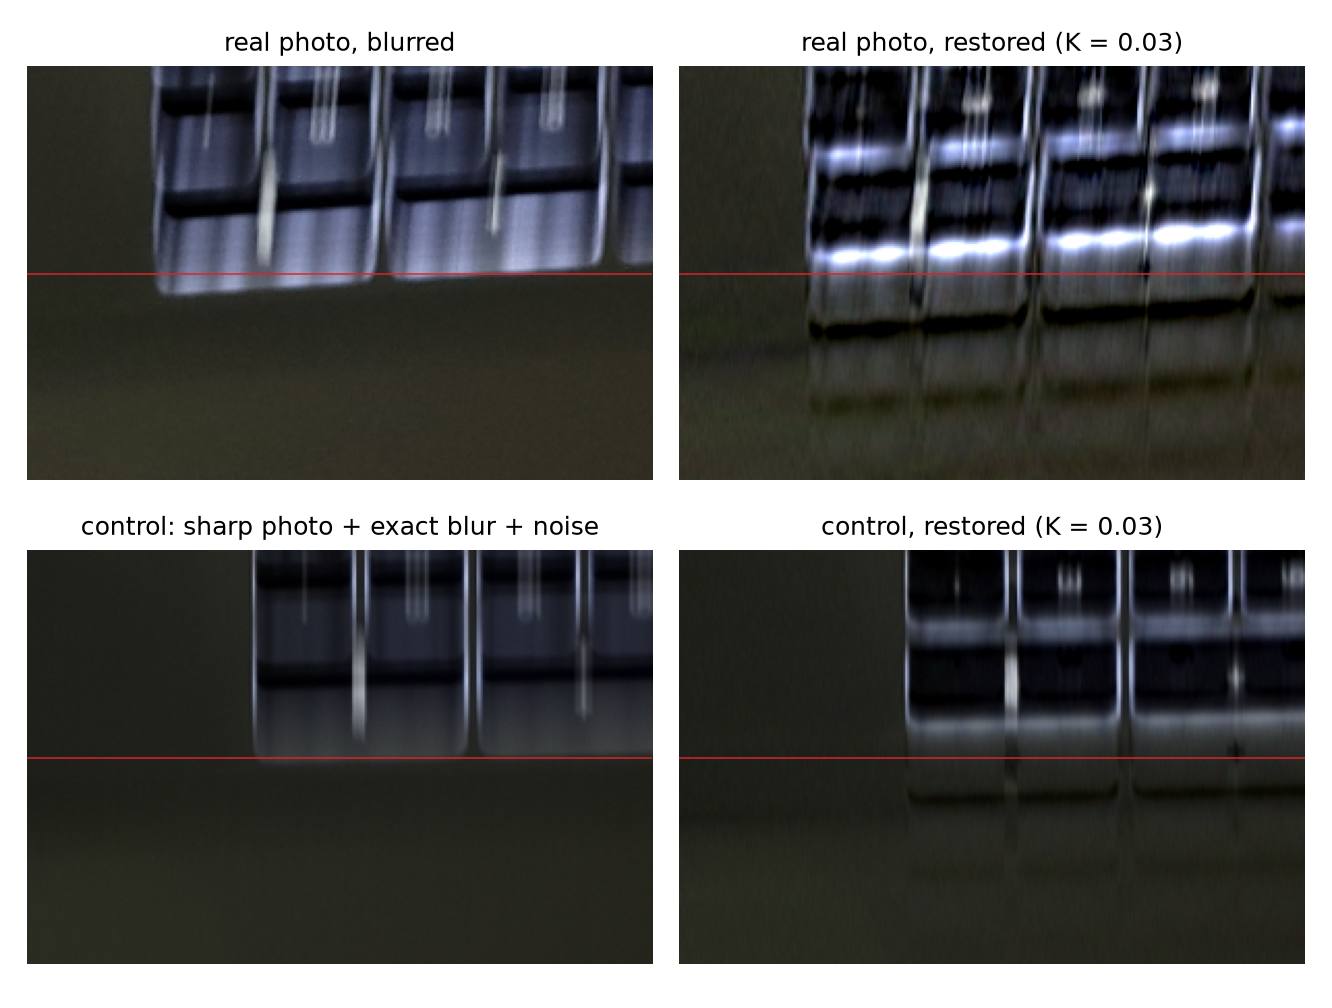
\includegraphics[width=\linewidth]{problem_6/real_blur_echo.png}
\caption{Bands below the brightest edge. From left: the blurred photo and its
restoration ($K=0.03$), and the control (my sharp photo of the keyboard blurred
with the estimated PSF plus white noise at the photo's level) and its restoration.
The red line marks the edge; both restorations show a dark band about 20 rows and a
bright band about 40 rows below it (24 and 40 rows in the photo, 18 and 38 in the
control).}
\label{fig:real-echo}
\end{figure}

\begin{figure}[H]
\centering
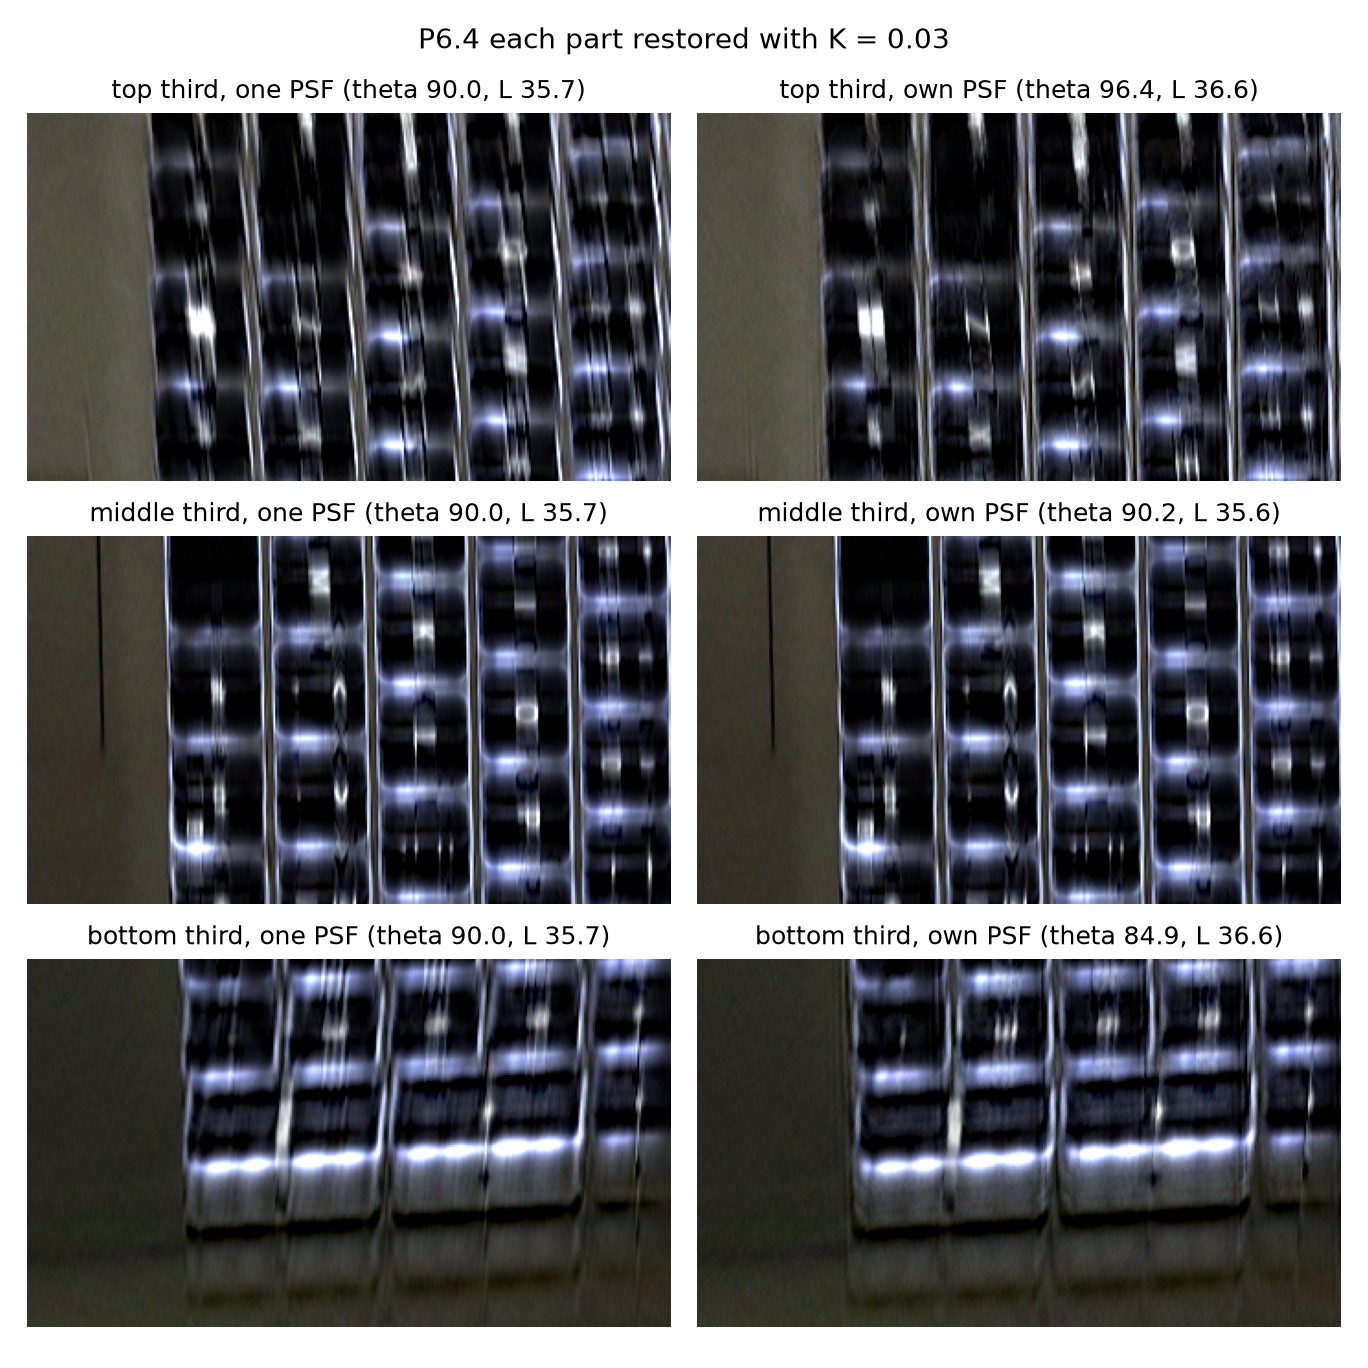
\includegraphics[width=\linewidth]{problem_6/real_blur_regions.png}
\caption{Top row: crops from the top, middle and bottom thirds of the blurred
photo, with the blur direction and length estimated on each third. Middle row: the
same crops restored with the single global PSF ($\theta=90.0^\circ$, $L=35.7$,
$K=0.03$). Bottom row: each third restored with its own estimated PSF. The middle
third is restored best; the top third keeps streaks with either PSF.}
\label{fig:real-regions}
\end{figure}
